\cotefile{50}
\scanpage{2}

Sur bouquin Lang

% archive sheet number: 1

\scanpage{3}

\[
\deleted{\mathrm{N\acute eron}(\unsure{/|1}\quad A\longrightarrow}
\]
\[
\text{\uuline{Néron}}_{A/S}\longrightarrow
\text{\uuline{Hom}}_{S\text{-}\mathrm{gr}}(A,A^*)
\]
\diagram{\begin{tikzcd}[ampersand replacement=\&,column sep=small,row sep=small]
{} \& \overset{s}{A}\times\overset{x}{A}\arrow[d,"\pi"] \& {}\\
(T_s)_*(\xi)-\xi \& A \& x\longrightarrow x-s
\end{tikzcd}}

\[
\deleted{A\mathrel{\unsure{-|\longrightarrow}}D^*}
\]
\[
\unsure{V|\vee}\qquad s\times A\qquad s_*\xi-\xi
\]
% slanted, left of the box
\figure{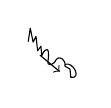
\begin{tikzpicture}[x=.52cm,y=.52cm,line cap=round,line join=round]
\draw (0,0) -- (.05,.32) -- (.12,-.02) -- (.19,.12) -- (.23,-.23) -- (.31,-.12) -- (.33,-.35) .. controls (.44,-.11) and (.52,-.16) .. (.49,-.43) .. controls (.42,-.69) and (.68,-.53) .. (.68,-.45) .. controls (.78,-.32) and (.93,-.48) .. (.90,-.61) -- (1.01,-.67);
\draw[->] (.29,-.34) -- (.77,-.74);
\draw (.91,-.56) .. controls (1.09,-.49) and (1.32,-.92) .. (1.04,-.88) -- (1.02,-.68);
\end{tikzpicture}}

\[
\boxed{\pi^*(\xi)-\mathrm{pr}_1(\xi)-\mathrm{pr}_2(\xi)}
\]

(i) $\xi$ dans le noyau \deleted{$s^*\xi$} de $\text{\uuline{Pic}}_{A/S}^{\deleted{\unsure{\tau}}}\longrightarrow\text{\uuline{Hom}}(A,A^*)$, i.e. $s\xi=\xi$

(i$'$). $\pi^*(\xi)-\mathrm{pr}_1(\xi)-\mathrm{pr}_2(\xi)=0$
\margin{$s.D\sim D$}

(ii) $\xi\in\text{\uuline{Pic}}^\tau_{\deleted{\unsure{A/S}}}(A/S)$

(iii) $\xi\in\mathrm{Im}\,\mathrm{Ext}^{1}_{\deleted{\unsure{S|\xi}}}(A,\mathbb{G}_m)$

$(\mathrm{i})\iff(\mathrm{i}')$ trivial

$(\mathrm{ii})\iff(\mathrm{iii})$ par le raisonnement \inserted{\unsure{géométrique|giraudique}} de Serre

$(\mathrm{ii})\Longrightarrow(\mathrm{i})$ par la propriété additive de $\text{\uuline{Pic}}^\tau$

$(\mathrm{i})\Longrightarrow(\mathrm{ii})$ c'est le th. de Barsotti-Cartier-Serre —

% archive sheet number: 2

\scanpage{4}
\mspage{- 176 -}

n° 280

\[
v(x+y)=\inf\,(v(x),v(y)).
\]

La relation (5) se déduit de $(\mathrm{VA}_{\mathrm{II}})$ par récurrence sur $n$. S'il existe un seul indice $k$ tel que $v(x_k)=\inf_{1\leqslant i\leqslant n}(v(x_i))$, on peut écrire $x_i=y_i\,x_k$ avec $v(y_i)>0$ pour $i\ne k$ ; on en déduit $\sum_{i=1}^n x_i={}
=x_k(1+\sum_{i\ne k}y_k)=x_k(1+y)$ avec $v(y)>0$ ; si $A$ désigne l'anneau de $v$, on a $1+y\in A$ et $1+y\notin\mathfrak{m}(A)$, d'où $v(1+y)=0$ et $v(\sum_{i=1}^n x_i)=v(x_k)$.

\uline{Corollaire} - \uline{Si des éléments} $x_i$ \uline{de} $K$ $(1\leqslant i\leqslant n,\ n\geqslant 2)$ \uline{sont tels que} $\sum_{i=1}^n x_i=0$, \uline{il y a au moins deux indices} $j$ \uline{et} $k$ \uline{tels que} $v(x_j)={}
=v(x_k)=\inf_{1\leqslant i\leqslant n}(v(x_i))$.

S'il n'y avait qu'un seul indice $k$ avec $v(x_k)=\inf_{1\leqslant i\leqslant n}(v(x_i))$, la prop.4 montrerait que $v(x_k)=v(0)=+\infty$, d'où $v(x_i)=+\infty$ pour $1\leqslant i\leqslant n$ contrairement à l'hypothèse faite sur $k$.

2. - \uline{Traductions}

Soient $K$ un corps, $\varphi$ une place de $K$, $v$ une valuation de $K$, et $A$ un anneau de valuation pour $K$. Nous dirons que $A$, $\varphi$ et $v$ sont \uline{associés} si $A$ est l'anneau de $\varphi$ et l'anneau de $v$. En vertu du n°1 et du \S2, chacun des trois objets $A$, $\varphi$ et $v$ détermine alors les deux autres (à une équivalence près en ce qui concerne les places et les valuations)/ On a en particulier
\[
\begin{aligned}
x\in A &\Longleftrightarrow \varphi(x)\ne\infty &\Longleftrightarrow v(x)&\geqslant 0\\
x\in\mathfrak{m}(A) &\Longleftrightarrow \varphi(x)=0 &\Longleftrightarrow v(x)&>0\\
x\in A-\mathfrak{m}(A)&\Longleftrightarrow\varphi(x)\ne0\text{ et }\varphi(x)\ne\infty & v(x)&=0
\end{aligned}
\]

Tout résultat portant sur les anneaux de valuation, les places ou les valuations se traduit en un résultat portant sur les deux autres notions. Ainsi, la prop.4 du \S2 donne :

\uline{Proposition} 5 - \uline{Soient} $K$ \uline{un corps}, $F$ \uline{un sousècorps de} $K$, \uline{et} $v$ \uline{une valuation de} $F$. \uline{Il existe une valuation} $w$ \uline{de} $K$ \uline{dont la restriction à} $F$ \uline{est équivalente à} $v$.

% archive sheet number: 3

\scanpage{5}

% top edge torn through a letter
$\unsure{P|r}$

N.S.

% slanted
\margin{\deleted{\unsure{par}}}
\diagram{\begin{tikzcd}[ampersand replacement=\&,column sep=2pt,row sep=9pt]
{} \& \text{torsion}\arrow[d,Rightarrow,shift left=4pt,"{\substack{\text{additivité}\\\text{de }\text{\uuline{Pic}}^\tau,\ \text{ou}\\\text{\unsure{raison} spéciale :}\\dA=A}}"] \& {} \& {}\arrow[dd,Rightarrow,"{\substack{\text{\unsure{trivial}}\\\text{par th.}\\\text{des \unsure{int}}}}"'] \& {} \\
{} \& {\equiv}\arrow[u,Rightarrow,shift left=5pt] \& {} \& {} \& {}\\
{} \& \text{équivalence numérique} \& {} \& {} \& {}\arrow[uu,Rightarrow,"{\substack{\text{th. non trivial}\\\text{\unsure{valable} pour les}\\\text{var. non sing}\\\text{projectives}}}"']
\end{tikzcd}}

[critère de Weil. \inserted{\tikz[baseline=(a.base)]\node[draw,rounded corners=7pt,inner sep=2pt](a){\unsure{dû|oui} à Matsusaka};} -]

Il y a une \unsure{dém.} directe plus simple pour les VA (bouquin Lang)

\diagram{\begin{tikzcd}[ampersand replacement=\&,column sep=3pt,row sep=4pt]
|[draw,inner sep=3pt]|{\begin{array}{lc}
\text{algébrique}&\Downarrow\\
\text{torsion}&\Downarrow\\
\equiv&{}\\ \hline
\text{numérique}&{}
\end{array}} \& {\Big\Uparrow\ \Big/\!\Big/} \&
{\displaystyle \leqslant\dim\mathrm{Pic}\,A
\underset{\substack{\text{\deleted{\unsure{théorème}} \inserted{déf.} de Picard ;}\\
\text{égalité ssi}\\\mathrm{Pic}\,A\text{ non}\\\text{singulier}}}{\leqslant}
\dim H^{1}(A,\uline{\unsure{\mathcal O|\mathrm O}}_A)
\underset{\substack{\text{th. de}\\\text{Hopf-Borel}}}{\leqslant}n}
\end{tikzcd}}

\diagram{\begin{tikzcd}[ampersand replacement=\&]
|[draw,rounded corners=16pt,inner sep=5pt]|{\displaystyle
\dim A\overset{\substack{\text{théorie des}\\\text{diviseurs non}\\\text{dégénérés}}}{\leqslant}
\dim\mathrm{Pic}\,A\overset{\text{déf. de Picard}}{\leqslant}
\dim H^1(A,\mathcal O_A)\overset{\text{Hopf-Borel}}{\leqslant}\dim A}
\end{tikzcd}}

\[
A^{**}\quad A\enspace .\quad A^*
\]

\figure{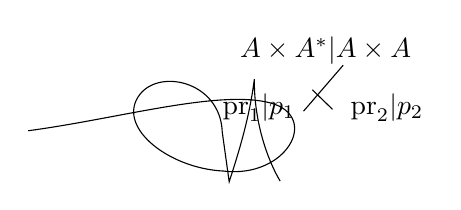
\begin{tikzpicture}[x=.8cm,y=.8cm,line width=.4pt]
\draw (0,.28) .. controls (1.43,.47) and (3.03,.94) .. (3.85,.72) .. controls (4.64,.5) and (4.1,-.48) .. (3.1,-.36) .. controls (2.25,-.32) and (1.43,.31) .. (1.74,.81) .. controls (2.03,1.29) and (3.05,1.08) .. (3.08,.26) -- (3.19,-.53) .. controls (3.39,.08) and (3.52,.56) .. (3.59,1.10) .. controls (3.58,.53) and (3.75,-.10) .. (4.0,-.52);
\node at (4.72,1.55) {$\unsure{A\times A^*|A\times A}$};
\node at (4.68,.65) {$\unsure{\mathrm{pr}_1|p_1}\qquad\unsure{\mathrm{pr}_2|p_2}$};
\draw (4.37,.59) -- (5.00,1.32);
\draw (4.51,.93) -- (4.83,.62);
\end{tikzpicture}}

% archive sheet number: 4

\scanpage{6}

% The torn edge cuts across the ends of the first three surviving lines.
$v_A:K^*\longrightarrow\Gamma_A$ est s\unsure{urje}\illegible{1}

Soit maintenant $v=K^*\longrightarrow\Gamma$ une valuati\unsure{on}\illegible{4} l'ensemble des $x\in K$ tels que $v(x)\geqslant0$. Si $x\in A$ et $y\in$ \illegible{4} $xy\in A$, $-x\in A$ ; en outre, $1\in A$ ; donc $A$ est un sous-anneau de $K$ (contenant 1). Si $x\in K$ et $x\notin A$, on a $v(x)<0$, d'où $v(x^{-1})>0$ et $x^{-1}\in A$ Donc $A$ est un anneau de valuation pour $K$. Les élément inversibles de $A$ forment un groupe $U$ qui est l'ensemble des $x\in K^*$ pour lesquels $v(x)=0$. On peut donc factoriser $v$ sous la forme $v=\sigma\mathbin{\unsure{\mathrm{o}|\circ}}v_A$, où $\sigma$ est un homomorphisme injectif de $\Gamma_A$ dans $\Gamma$. Si $\xi=(x)$ est un élément $\geqslant0$ de $\Gamma_A$, on a $x\in A$, d'où $\sigma(x)=v(x)\geqslant0$ ; donc $\sigma$ est croissant, ce qui achève de prouver la prop.3 .

La factorisation $v=\sigma\circ v_A$ est appelée la \uline{factorisation canonique} de $v$. On dit que $A$ est \uline{l'anneau de la valuation} $v$ (d'où la terminologie d'anneau de valuation), que $\mathfrak{m}(A)$ est \uline{l'idéal de} $v$, et que $\unsure{\varkappa|\mathfrak{k}|x}_A$ est le \uline{corps résiduel de} $v$. Le sous-groupe $\sigma(\Gamma_A)=v(K^*)$ est appelé le \uline{groupe des ordres de} $v$. Pour $x\in K$, l'élément $v(x)$ est parfois appelé la valuation ou l'ordre de $x$ (A vider ! ! ). Deux valuations $v$ et $v'$ sont dites \uline{équivalentes} si elles ont même anneau de valuation ; pour cela, il faut et il suffit, en vertu de la prop.3, qu'il existe un isomorphisme $\lambda$ du groupe ordonné $v(K^*)$ sur le groupe ordonné $v'(K^*)$ tel que $v'=\lambda\circ v$.

\uline{Proposition} 4 - \uline{Soit} $v$ \uline{une valuation d'un corps} $K$. \uline{Quels que soient} $x_i\in K$ $(1\leqslant i\leqslant n)$, \uline{on a}
\[
v(\sum\nolimits_{i=1}^n x_i)\geqslant\inf\nolimits_{1\leqslant i\leqslant n}(v(x_i))\tag*{(5)}
\]

Si en outre il existe un seul indice $k$ tel que $v(x_k)=\inf_{1\leqslant i\leqslant n}(v(x_{\unsure{i}}$
% right edge cuts off the end of this line
il y a alors égalité dans (5). En particulier, si $v(x)\ne v(y)$, on a

% archive sheet number: 5

\scanpage{7}

\uline{Th.} Soit $\xi\in N^{\deleted{\unsure{+|*}}>}(A)$, considérons l'involution
\[
\alpha\leadsto\alpha'=\deleted{\unsure{\varphi_\xi}}\varphi_\xi^{-1}\,{}^{t}\alpha\,\varphi_\xi
\]
de $\mathrm{Hom}(A,A)_{\mathbb Q}$, Alors \unsure{on a}
\[
\mathrm{tr}(\alpha\beta')=
\frac{r}{I(\xi,\cdots,\xi)}
I(\xi,\cdots,\xi,D_{\xi}(\alpha\beta'))
\]
d'où
\[
\mathrm{tr}\,\alpha\alpha'=
\frac{r}{I(\xi,\cdots\xi)}
I(\xi,\unsure{-|\cdots}\xi,2\alpha^*(\xi))
\]

\uline{Corollaire}

% archive sheet number: 6

\scanpage{8}

% slanted
\margin{après d)}
\textcircled{e} Pour tout $A\in\mathrm{ob}\,\unsure{\mathscr A|\mathcal A}$, on suppose qu'il y a \inserted{un entier $r=\dim(A)$} et une forme $r$-fois \uline{linéaire}
\[
(\xi_1,\deleted{\unsure{\xi|\cdots}},\xi_r)\leadsto
\deleted{\unsure{\varphi}}I(\xi_1,\cdots,\xi_r)\in\deleted{\mathbb Q}\mathbb Z
\]

2) On suppose $I$ \deleted{\unsure{pos}} str. pos. sur $N^+(A)$, i.e. $\xi_1,\cdots,\xi_r\in N^+(A)\Rightarrow I(\xi_1,\cdots,\xi_r)>0$.

% slanted
\margin{plus \unsure{généralement} si $u:A\longrightarrow B$ est un \unsure{morphisme} \deleted{\unsure{non}} \deleted{\unsure{tel que} $\unsure{u(A)\ne0}$ \illegible{3} \unsure{choisissant} \illegible{2} $\unsure{1\leqslant s\leqslant\dim A}$} \deleted{\unsure{de dim}} et $\eta_1\in N^{\unsure{>|+}}(B)$, alors \unsure{posant|pour} $\xi_1=u^{\unsure{-1|*}}(\eta_1)$, on a $I(\xi_1,\xi_2,\cdots\xi_r)>0$ pour $\xi_2\cdots\xi_r\in N^>(A)$}

3) On suppose que pour tout \unsure{morphisme} $u:A\longrightarrow B$ \deleted{qui est un $\mathbb Q$-isomorphisme, ou comme nous dirons, une \uline{isogénie}, on a $\unsure{r(A)=}$} avec $\dim(A)=\dim(B)$, \deleted{\unsure{et}} il existe un entier \deleted{\unsure{de}} $\unsure{\nu|v}(u)$ tel que
\[
\deleted{\unsure{\xi}} I(u^*(\xi_1),\cdots,u^*(\xi_r))=\nu(u)\,I(\xi_1,\cdots,\xi_r)
\]
pour \unsure{tt|$\forall$} système $\xi_1,\cdots,\xi_r$ [ce qui détermine $\nu(u)$ de façon unique]\deleted{, \unsure{et} cf. plus \unsure{haut}]} et que ($\dim\deleted{\unsure{\mathrm{Ker}\,u}}\inserted{A=\dim B},\ \nu(u)\ne0$) ssi $u$ est un $\mathbb Q$-isomorphisme (``une \uline{isogénie}'').

Prenant en particulier \deleted{$A=B$, et} un $\xi$ dans $N(\deleted{A}B)$ tel que $\varphi_{\unsure{\xi|\eta}}$ soit un isom et $I(\xi,\cdots,\xi)$ soit $>0$ [\deleted{\unsure{on}} \unsure{supposons|supposera} que 2) \unsure{pour cela existe|pour un certain $\xi$}] on \unsure{trouve}
\[
\nu(\alpha)=\frac{1}{I(\xi,\cdots\xi)}I(\alpha^*(\xi),\cdots,\alpha^*(\xi))
\]
$={}$ \uline{forme de degré} $2r$ \uline{en} $\alpha$ \inserted{à coefficients \unsure{entiers}}. Si $A=B$, on aura donc
\[
\nu(\alpha+n\unsure{1|\mathbb 1}_A)=n^{2r}+\deleted{\unsure{\mathrm{tr}}}\sigma_1(\alpha)n^{2r-1}+\cdots+\sigma_{2r}(\alpha)
\]
et on posera
\[
\sigma_1(\alpha)=\mathrm{tr}\,\alpha
\]
tandis qu'on a
\[
\sigma_{2r}(\alpha)=\nu(\alpha)\ ,\ \text{noté aussi }\det\alpha
\]

% archive sheet number: 7

\scanpage{9}

de façon générale, \deleted{$D_\xi(\alpha)$} $\sigma_i(\alpha)$ est une forme de degré $2i$ en $\alpha$, On a en particulier, par un calcul \unsure{facile}
\[
\mathrm{tr}(\alpha)=\frac{r}{I(\xi,\cdots,\xi)}I(\xi,\cdots,\xi,D(\alpha))
\]

\textcircled{d} Pour tout $A\in\mathrm{Ob}\,\unsure{\mathscr A|\mathcal A}$, on se donne deux parties
\[
N^{\unsure{>|+|\geqslant}}\ \deleted{\text{\unsure{et}}\ N^{\unsure{+|>}}}(A)\subset N(A)
\]
\deleted{$N^+(A)$ \unsure{tels} dépendent \unsure{de} \unsure{fonctoriellement} de $A$, et \unsure{vérifient}} \inserted{$N^>(A)$ dép. \unsure{fonctlt}} pour les \uuline{isogénies}, \unsure{ayant|vérifiant} les propriétés suivantes

% slanted
\margin{\deleted{$\xi\in N^+(A)$ : $\exists m>0$ tel que $m\xi$ soit représentable par un diviseur \uline{positif} $\iff$ $\xi$ est l'image inverse d'un \unsure{élt|élément} d'un $N^>(B)$ ; cela \unsure{dispense} donc d'introduire $N^{\unsure{+|>}}(A)$ explicitement.}}

a) $N^>(A)+N^>(A)\subset N^>(A)$, \deleted{\unsure{et}} $m>0\Rightarrow mN^>(A)\subset N^>(A)$
\inserted{Kif Kif pour $N^{\unsure{\geqslant|>}}(A)$}

b) $N^>(A)$ engendre $N(A)$

\deleted{c) $\xi\in N^+(A)\Longrightarrow I$ est $>0$ sur $N^+(A)$, i.e. $\xi_1,\cdots\xi_r\in N^+(A)\Rightarrow I(\xi_1,\cdots\xi_r)>0$}

c) $\xi\in N^>(A)\Longrightarrow\varphi_\xi$ \unsure{$\xi$} est un $\mathbb Q$-isom :

% archive sheet number: 8

\scanpage{10}

qui d'ailleurs s'annule sur $\mathrm{Im}\,N(A)+\mathrm{Im}\,N(B)$

\uline{Propriétés fondamentales} 1) On trouve ainsi un \uline{isom}
\[
N(A\times B)/N(A)\times N(B)\xrightarrow{\sim}\mathrm{Hom}(A,D(B))
\]
% slanted
\margin{\uline{purement} \uline{formel}}

\deleted{2) Pour tout $A$, il existe des $\xi\in N(A)$ telles \deleted{\unsure{Pour}} que $\varphi_\xi:A\xrightarrow[\otimes\mathbb Q]{\sim}D(A)$ [\unsure{N.B. Cela|N.B. on} suppose \unsure{qu'on} a \unsure{tensorisé} les $\mathrm{Hom}$ de var. ab. par $\mathbb Q$]}

\inserted{Si $\varphi_\xi:A\longrightarrow D(A)$ est un $\mathbb Q$-isom,} Cela permet donc de définir une involution sur $\mathrm{Hom}_{\mathbb Q}(A,A)$ par
\[
s_\xi(\alpha)=\varphi_\xi^{-1}\,{}^t\alpha\,\varphi_\xi
\]

\uline{C'est là une involution} \uline{\deleted{\unsure{de l'algèbre}}} \uline{l'anneau} $\mathrm{Hom}(A,A)$

Posons pour $\alpha,\beta\in\mathrm{Hom}_{\mathbb Q}(A,A)$
\[
D_\xi(\alpha,\beta)=(\alpha+\beta)^*(\xi)-\alpha^*(\unsure{\eta|\xi})-\beta^{\unsure{*|\alpha}}(\xi)\in N(A)\quad\text{i.e.}
\tag*{(1)}
\]
\[
\varphi_{D_\xi(\alpha,\beta)}={}^{t}(\alpha+\beta)\varphi_\xi(\alpha+\beta)-{}^{t}\unsure{\alpha|d}\,\varphi_\xi\alpha-{}^{t}\beta\varphi_\xi\beta\qquad\text{\unsure{i-e|i.e}}
\]
\[
\begin{aligned}
\varphi_{D_\xi(\alpha,\beta)}&={}^{t}\beta\varphi_\xi\alpha+{}^{t}\alpha\varphi_\xi\beta\\
&=\varphi_\xi(\alpha'\beta+\beta'\alpha)
\end{aligned}\tag*{(1\ensuremath{^{\prime}})}
\]

(où on pose pour \unsure{abréger|désigner} $\alpha'=s_\xi(\alpha)$) ; \deleted{\unsure{d'où}}

posons aussi
\[
D_\xi(\alpha)=D_\xi(\alpha,\mathrm{id}_A)=\varphi_\xi(\alpha'+\alpha)\qquad\text{d'où}
\tag*{(2)}
\]
\[
D_\xi(\alpha,\beta)=D_\xi(\alpha'\beta)=D_\xi(\beta'\alpha)\ ,\quad D_{\unsure{\xi}}(\alpha)=D_\xi(\alpha')
\tag*{(3)}
\]

% archive sheet number: 9

\scanpage{11}
\margin{livre de Lang\\ VA}
\textcircled{a}\quad Catégorie additive $\unsure{\mathscr A|\mathcal A}$

\textcircled{b}\quad Autodualité.
\[
 D:\mathscr A^{\unsure{o|\circ}}\longrightarrow\mathscr A
\]
(munie d'un isom
\[
 \unsure{k|\kappa}:\mathrm{id}_{\mathscr A}\longrightarrow D\circ D
\]
satisfaisant la condition de compatibilité habituelle).

\unsure{,} Soit alors
\[
 \unsure{\mathcal B|B}(A,B)=\mathrm{Hom}(A,D(B))
 \xrightarrow{\overset{s}{\sim}}\mathrm{Hom}(B,D(A))
\]
c'est un bifoncteur contravariant en $A,B$. On suppose de plus

\textcircled{c}\quad Pour tt $A\in\mathrm{Ob}\,\mathscr A$, un sous-groupe
\[
 \boxed{N(A)\subset B(A,A)^{\unsure{\text{antisymm}|\text{antisym}}}}
\]
dépendant de $A$ de façon\deleted{\illegible{1}} contravariante.
[N.B. $N$ n'est pas additif en $A$ ...]

Si $\xi\in N(A)$, on pose aussi $\varphi_\xi:A\longrightarrow D(A)$
le morphisme qu'il définit.

Soit $\xi\in N(A\times B)$, il définit
\[
 \varphi_{\xi}: A\times B\longrightarrow D(A)\times D(B)
\]
qui est antisym\uline{étrique}, donc \unsure{nécessairem|nécessairement} de
la forme
\[
 \begin{aligned}
 \begin{pmatrix}\alpha_\xi&{}^t\lambda_\xi\\-\lambda_\xi&\beta_\xi\end{pmatrix},
 &\quad \lambda_\xi\in\mathrm{Hom}(A,D(B))=B(A,B)\\
 &\quad \alpha_\xi\in B(A,A),\ \beta_\xi\in B(\deleted{\unsure{A}}B,B)
 \end{aligned}
\]
on obtient ainsi un hom
\[
 \boxed{\xi\leadsto\lambda_\xi:\ N(A\times B)\longrightarrow
 \mathrm{Hom}(A,D(B))=B(A,B)}
\]
% archive sheet number: 10

